%+TITLE: Los solitones topológicos más simples
%+DESCRIPTION: El kink, los argumentos de escala para soluciones estáticas y el vórtice en una teoría de gauge U(1).
% Traducción de las seis páginas del manuscrito. Las expresiones dudosas se
% conservan y se señalan con comentarios numerados de REVISIÓN.
\documentclass[11pt,a4paper]{article}

\usepackage{babel}
\babelprovide[import=es,main]{spanish}
\usepackage{amsmath,amssymb}
\usepackage{graphicx}
\usepackage{geometry}
\usepackage{enumitem}
\usepackage{microtype}
\usepackage{mathtools}
\usepackage[most]{tcolorbox}
\definecolor{infobg}{gray}{0.94}
\newtcolorbox{info}[1][]{%
  enhanced,
  breakable,
  colback=infobg,
  colframe=infobg,
  boxrule=0pt,
  arc=0pt,
  outer arc=0pt,
  left=6pt,
  right=6pt,
  top=6pt,
  bottom=6pt,
  before skip=0.75\baselineskip,
  after skip=0.75\baselineskip,
  parbox=false,
  #1}

% Shared math macros for notes written directly in LaTeX.
%
% These are used natively when compiling a PDF and are expanded by pandoc
% when building the website, so MathJax never needs to know about them.
% Prefer plain \newcommand definitions: pandoc expands those reliably,
% including inside math and with arguments. Exotic macros (\def, xparse,
% optional arguments) may not be expanded -- see AGENT.md.

\newcommand{\dd}{\mathrm{d}}
\newcommand{\vv}[1]{\mathbf{#1}}
\newcommand{\PL}{P_{\mathrm{L}}}
\newcommand{\avg}[1]{\langle #1 \rangle}


\geometry{margin=2.3cm}
\setlength{\parindent}{0pt}
\setlength{\parskip}{0.65em}
\setlist[itemize]{leftmargin=1.6em,itemsep=0.25em,topsep=0.25em}
\newcommand{\Tr}{\operatorname{Tr}}

\begin{document}

% Página 1 del manuscrito
\section*{El kink}

% REVISIÓN 1. Falta 1/2 en el término cinético para obtener las
% ecuaciones siguientes con la normalización canónica. Con la métrica
% de las clases anteriores el término es -\partial_\nu\varphi\partial^\nu\varphi/2.
% REVISIÓN 2. La igualdad de los dos potenciales requiere \mu^4/(4\lambda)
% como término constante, en vez de \mu^2/(4\lambda).
\begin{align*}
S &= \int \dd^2x\,\bigl[(\partial_\nu\varphi)^2 - V(\varphi)\bigr],
& \nu &= 0,1,\\
V(\varphi) &= -\frac{\mu^2}{2}\varphi^2
  + \frac{\lambda}{4}\varphi^4 + \frac{\mu^2}{4\lambda}
  = \frac{\lambda}{4}(\varphi^2-v^2)^2,
& v &= \frac{\mu}{\sqrt{\lambda}}.
\end{align*}

La acción $S$ es invariante bajo $\varphi\to-\varphi$ y hay dos vacíos,
en $\varphi^{(v)}=\pm v$. Las excitaciones lineales alrededor de estos
vacíos tienen masa $m=\sqrt{2}\,\mu$.

Tomemos $\lambda\ll\mu^2$, es decir, $v\gg1$. Consideremos una partícula
de masa $m$ y energía $E\sim m$:
\[
E=\int\dd x\,
  \left[\frac12(\Delta\dot{\varphi})^2
  +\frac12(\Delta\varphi')^2+\frac{m^2}{2}(\Delta\varphi)^2\right],
\qquad \Delta\varphi\equiv\varphi-v.
\]
La partícula ocupa una región del orden de su longitud de onda de Compton,
$\dd x\sim1/m$, de modo que
% REVISIÓN 3. La energía cuadrática da E\sim m(\Delta\varphi)^2.
\[
E\sim m\,\Delta\varphi \quad\Rightarrow\quad \Delta\varphi\sim1.
\]
Por tanto, si $v\gg1$, los desplazamientos respecto del vacío son pequeños,
$\Delta\varphi\ll v$.

Un kink es una solución estática que interpola entre $\varphi=-v$ en
$x=-\infty$ y $\varphi=v$ en $x=\infty$.

\begin{center}
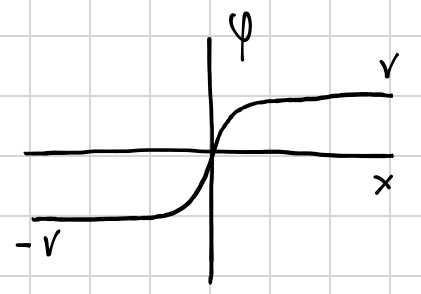
\includegraphics[width=0.23\linewidth]{figures/perfil-kink.png}
\end{center}

Esta solución tiene energía finita. En efecto,
\[
E=\int\dd x\,
  \left[\frac12\left(\frac{\dd\varphi}{\dd x}\right)^2
  +\frac{\lambda}{4}(\varphi^2-v^2)^2\right],
\]
% REVISIÓN 4. Que ambos términos tiendan a cero no garantiza integrabilidad.
% El perfil explícito que se obtiene abajo da un decaimiento exponencial.
y ambos términos tienden a cero cuando $x\to\pm\infty$.

La ecuación de campo es $\varphi''-\partial V/\partial\varphi=0$.
Tiene la forma de la ecuación de una partícula newtoniana con tiempo $x$,
potencial $-V$ y posición $\varphi$.

El kink es la trayectoria de esta partícula que parte en $-v$ en el pasado
infinito y llega a $+v$ en el futuro infinito. La energía de esta partícula es
\[
\mathcal{E}_0=\frac12\varphi'^2-V(\varphi).
\]
Como $\varphi'\to0$ y $V(\varphi)\to0$ cuando $x\to\pm\infty$, tenemos
$\mathcal{E}_0=0$. Entonces
\begin{align*}
\frac{\dd\varphi}{\dd x}
  &= \sqrt{2V}=\sqrt{\frac{\lambda}{2}}(v^2-\varphi^2)
\\
&\Rightarrow\quad
\varphi=v\tanh\left(\sqrt{\frac{\lambda}{2}}\,v(x-x_0)\right)
  =\frac{\mu}{\sqrt{\lambda}}\tanh\left(\frac{\mu}{\sqrt{2}}(x-x_0)\right).
\end{align*}

% Página 2 del manuscrito
Algunas observaciones:
\begin{itemize}
\item El tamaño del kink es $r_k\sim\mu^{-1}\sim m^{-1}$, es decir, la
  longitud de onda de Compton de una partícula elemental. La energía del
  kink se concentra en la región $|x|\lesssim r_k$.
\item La energía estática del kink es
  \begin{align*}
  E_k&=\int_{-\infty}^{\infty}\dd x\,
      \left(\frac12\varphi'^2+V(\varphi)\right)\\
    &=\int_{-\infty}^{\infty}\dd x\,
      \frac{\lambda}{2}v^4\frac{1}{\cosh^4(\frac{\mu}{\sqrt{2}}x)}
    =\frac23mv^2.
  \end{align*}
  Esta es la masa del kink. Como $v\gg1$, su tamaño es mucho mayor que
  su propia longitud de onda de Compton y su masa es mucho mayor que la
  de una excitación elemental.
\item Para $|x|$ grande, $\varphi\approx v-2v e^{-mx}$, de modo que
  $\varphi$ satisface la ecuación estática de Klein--Gordon (decaimiento
  exponencial).
  % REVISIÓN 5. Con x_0=0 la expresión escrita vale para x\to+\infty.
  % Para x\to-\infty se tiene \varphi\approx-v+2v e^{mx}.
\item Las traslaciones y los boosts no dejan invariante esta solución.
  Un boost da un kink en movimiento,
  \[
  \varphi_k(x-x_0;t;v)
    =\frac{\mu}{\sqrt{\lambda}}
    \tanh\left(\frac{\mu}{\sqrt{2}}\frac{(x-x_0)-ut}{\sqrt{1-u^2}}\right).
  \]
  % REVISIÓN 6. En la lista de argumentos aparece v, pero la velocidad
  % en la expresión es u. En el resto de la clase v es el valor de vacío.
\end{itemize}

Estudiemos ahora la estabilidad de estas soluciones bajo perturbaciones pequeñas:
\[
\varphi(x,t)=\varphi_k(x)+\phi(x,t).
\]
% REVISIÓN 7. El manuscrito escribe ambos índices abajo en
% \partial_\mu\partial_\mu. La contracción lorentziana requiere subir uno.
\begin{align*}
-\partial_\mu\partial_\mu\varphi-\frac{\partial V}{\partial\varphi}=0
&\quad\Rightarrow\quad
-\partial_\mu\partial_\mu(\varphi_k+\phi)
-\frac{\partial V}{\partial\varphi}(\varphi_k)
-\frac{\partial^2V}{\partial\varphi^2}(\varphi_k)\phi+\dots=0\\
&\quad\Rightarrow\quad
-\partial_\mu\partial_\mu\phi
-\frac{\partial^2V}{\partial\varphi^2}(\varphi_k)\phi=0.
\end{align*}
Con $\phi(x,t)=e^{i\omega t}\phi_\omega(x)$,
\begin{align*}
\omega^2\phi_\omega+\phi_\omega''
  -\frac{\partial^2V}{\partial\varphi^2}(\varphi_k)\phi_\omega&=0,\\
\frac{\partial^2V}{\partial\varphi^2}(\varphi_k)
  &=\mu^2\left[3\tanh^2\left(\frac{\mu}{\sqrt{2}}x\right)-1\right].
\end{align*}

Se resuelve entonces para $\omega^2$. Si todos sus valores son
$\geq0$, la solución es estable. Al pasar al espacio de Fourier en $x$,
vemos que esto se cumple en este caso.
% REVISIÓN 8. V''(\varphi_k(x)) depende de x, así que la transformada de
% Fourier mezcla modos. La positividad se puede demostrar factorizando
% H=-\partial_x^2+V''(\varphi_k)=A^\dagger A con
% A=\partial_x-\varphi_k''/\varphi_k'.

Notemos que también hay un autovalor nulo, con autofunción
$\phi_{\omega=0}=\partial\varphi_k(x)/\partial x$, ya que
\[
-(\varphi_k')''+\frac{\partial^2V}{\partial\varphi^2}(\varphi_k)\varphi_k'
  =\frac{\partial}{\partial x}
   \left(-\varphi_k''+\frac{\partial V}{\partial\varphi}(\varphi_k)\right)
  =0.
\]
Esto se debe a la invariancia bajo traslaciones, pues $\varphi_k(x+a)$
también es una solución. Aparecerán otros modos cero si la solución
clásica rompe otras simetrías, sean del espacio-tiempo o internas.

Para discutir el carácter topológico, notemos que podemos asignar los
valores de vacío a los puntos del infinito de varias maneras:
\begin{center}
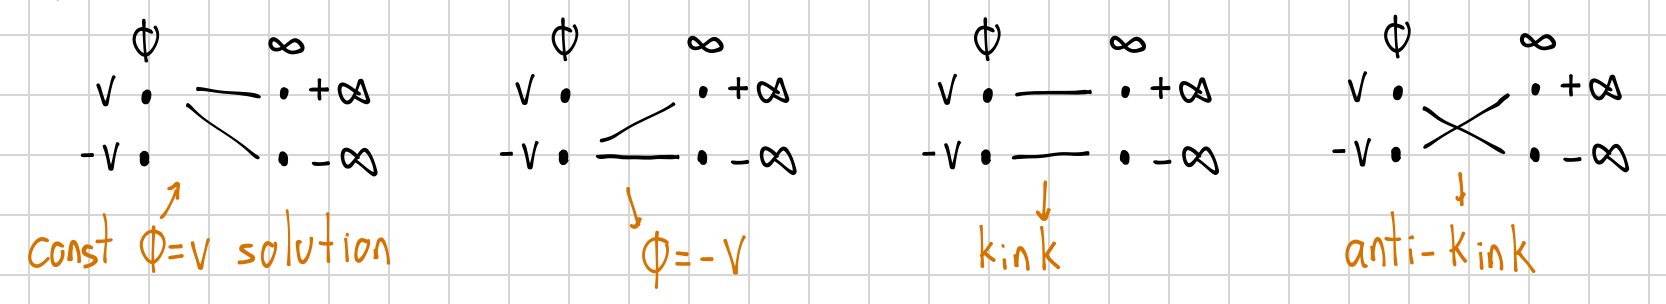
\includegraphics[width=0.94\linewidth]{figures/sectores-del-kink.png}
\end{center}

% Página 3 del manuscrito
La existencia del kink está asociada a una topología no trivial.

Definimos una \emph{corriente topológica}
\[
k^\mu=\frac{1}{2v}\epsilon^{\mu\nu}\partial_\nu\phi,
\]
que se conserva trivialmente. La \emph{carga topológica} es
\[
Q_T=\int_{-\infty}^{\infty}\dd x\,k^0
 =\frac{1}{2v}\int_{-\infty}^{\infty}\dd x\,\partial_x\phi
 =\frac{1}{2v}\bigl(\phi(+\infty)-\phi(-\infty)\bigr).
\]
Para el kink, $Q_T=+1$. Estas definiciones son útiles en configuraciones
menos triviales.

Una pared de dominio es una solución en tres dimensiones espaciales que
solo depende de una de ellas y tiene un perfil de kink.

\section*{Transformaciones de escala y teoremas sobre la ausencia de solitones}

Consideremos una teoría de $n$ campos escalares en $d+1$ dimensiones:
% REVISIÓN 9. Verificar los signos del término cinético escalar en los
% lagrangianos de esta sección y del vórtice con la métrica (-,+,+,+)
% usada en el curso. Para los términos de traza hay que fijar además
% si los generadores de gauge son hermíticos o antihermíticos.
\[
\mathcal{L}=\frac12 F_{ab}\,\partial_\mu\phi^a\,\partial^\mu\phi^b
   -V(\phi).
\]
Para una solución estática, la energía es
\[
E[\phi]=\int\dd^d x\,
  \left(\frac12 F_{ab}\,\partial_i\phi^a\,\partial^i\phi^b+V(\phi)\right).
\]

Para que $E$ esté acotada inferiormente, $F_{ab}$ debe ser definida positiva
y podemos fijar $V(\varphi^{(v)})=0$ de modo que $V(\varphi)\geq0$.

Una solución clásica estática $\varphi_c^a(\vec{x})$ debe hacer estacionaria
$E$ frente a variaciones que se anulan en el infinito. Consideremos la
transformación de escala
\[
\varphi_\lambda^a(\vec{x})=\varphi_c^a(\lambda\vec{x}).
\]
Para $\lambda$ cercano a $1$, $\varphi_\lambda^a(\vec{x})-\varphi_c^a(\vec{x})$
es pequeña y se anula en el infinito, pues de lo contrario la contribución
de los gradientes a $E$ divergiría. Por tanto,
\[
\left.\frac{\dd E}{\dd\lambda}\right|_{\lambda=1}=0,
\qquad E(\lambda)\equiv E[\varphi_\lambda].
\]
Pero
% REVISIÓN 10. En la primera integral los dos campos llevan a. El
% segundo campo debe llevar b para contraerlo con F_{ab}.
\begin{align*}
E(\lambda)
 &= \int\dd^d x\,\biggl(
     \frac12 F_{ab}(\varphi_c(\lambda\vec{x}))
       \partial_i\varphi_c^a(\lambda\vec{x})\,
       \partial^i\varphi_c^a(\lambda\vec{x})
       +V(\varphi_c(\lambda\vec{x}))\biggr)\\
 &= \int\dd^d y\,\lambda^{-d}\biggl(
     \frac12\lambda^2 F_{ab}(\varphi_c(\vec{y}))
       \frac{\partial\varphi_c^a(\vec{y})}{\partial y^i}
       \frac{\partial\varphi_c^b(\vec{y})}{\partial y_i}
       + V(\varphi_c(\vec{y}))\biggr)\\
 &= \lambda^{2-d}\Gamma+\lambda^{-d}\Pi,
 \qquad \Gamma\geq0,\quad\Pi\geq0.
\end{align*}
Por tanto, la condición es
\[
(2-d)\Gamma-d\Pi=0.
\]

% Página 4 del manuscrito
Para $d>2$ la única posibilidad es $\Pi=\Gamma=0$, de modo que la única
solución estática es el vacío clásico.

Para $d=2$ la condición es $\Pi=0$. Si $V$ no es constante, esto quiere decir
que la única solución estática es el vacío clásico. Otra posibilidad es
que $V=0$ en todas partes.
% REVISIÓN 11. Para d=2, \Pi=0 solo exige que el campo tome valores
% en V^{-1}(0). Que V no sea constante no implica que ese conjunto
% sea discreto.

Para $d=1$ podemos tener $\Gamma=\Pi$ (teorema del virial).

Consideremos ahora teorías de gauge.
\[
\mathcal L=\frac{1}{2g^2}\Tr F_{\mu\nu}F^{\mu\nu}
  +(D_\mu\phi)^\dagger(D^\mu\phi)-V(\phi).
\]
Busquemos soluciones estáticas en el gauge $A_0=0$. Entonces
\[
D_0\phi=0,\qquad F_{0i}=0.
\]
Buscamos extremos de la energía
\[
E[\phi,A]=\int\dd^d x\,
  \left(-\frac{1}{2g^2}\Tr F_{ij}F^{ij}
        +D_i\phi^\dagger D^i\phi+V(\phi)\right).
\]
Al reescalar $\phi_\lambda(\vec{x})=\phi_c(\lambda\vec{x})$ y
$\vec{A}_\lambda(\vec{x})=\lambda\vec{A}_c(\lambda\vec{x})$, los dos
términos de la derivada covariante escalan de la misma manera.
Entonces $F_{ij}$ se transforma como $F_{ij}\mapsto\lambda^2F_{ij}(\lambda\vec{x})$.
Por tanto,
\[
E=\lambda^{4-d}G+\lambda^{2-d}\Gamma+\lambda^{-d}\Pi,
\qquad G,\Gamma,\Pi\geq0.
\]
Así,
\[
(4-d)G+(2-d)\Gamma-d\Pi=0.
\]
No hay restricciones para $d\leq3$. Para $d=4$ necesitamos
$\Gamma=\Pi=0$. Para $d>4$ no se admiten soluciones estáticas.
% REVISIÓN 12. La condición sí restringe los términos para d\leq3.
% Para d=2 exige G=\Pi y para d=1 se tiene F_{ij}=0 y \Gamma=\Pi.
% Para d>4 el argumento excluye soluciones con energía no nula.

\section*{El vórtice}

Consideremos una teoría de gauge $U(1)$ con un potencial de Higgs:
\[
\mathcal L=-\frac14F_{\mu\nu}^2+(D_\mu\varphi)^*(D^\mu\varphi)-V(\varphi),
\qquad V(\varphi)=\frac{\lambda}{2}(|\varphi|^2-v^2)^2,
\]
con $\mu=\sqrt{\lambda}\,v$. El campo $A_\mu$ tiene masa $m_V=\sqrt{2}\,ev$.
Trabajemos en el gauge $A_0=0$. La energía de una solución estática es
% REVISIÓN 13. Aquí se integra en tres dimensiones, pero para un vórtice
% recto en 3+1 la integral transversal que sigue da energía por unidad
% de longitud. En 2+1 esa integral da la energía total.
\[
E[\phi,A_\mu]=\int\dd^3 x\,
  \left[\frac14 F_{\mu\nu}F^{\mu\nu}+D_i\phi^* D_i\phi+V(\phi)\right].
\]
Para que la energía sea finita es necesario que la densidad de energía
tienda a cero en el infinito. En particular,
\[
|\varphi|\to v\qquad\text{cuando }\vec{x}\to\infty.
\]
Podemos tener $\varphi=v e^{if(\theta)}$ cuando $\vec{x}\to\infty$.
Esto define una aplicación entre el espacio de campos y el círculo en el
infinito.

% Página 5 del manuscrito
La fase del campo depende del gauge, pero el número de enrollamiento es
invariante. En efecto, si intentamos reducirlo,
\[
e^{i\alpha(\theta)}=e^{-i\theta}.
\]
Pero entonces $A_i'=A_i-\frac{1}{e}\partial_i\alpha$ diverge en el origen.
% REVISIÓN 14. Este signo corresponde a D_i=\partial_i+ieA_i para
% \varphi'=e^{i\alpha}\varphi. El A_i asintótico escrito abajo y el
% convenio de la clase 17 corresponden al signo opuesto en D_i.

El número de enrollamiento se puede definir como
% REVISIÓN 15. El manuscrito dice n^2 en el denominador; la fórmula
% siguiente requiere v^2, pues |\varphi|^2\to v^2 en el contorno.
\[
n=\frac{1}{2\pi i n^2}\oint_{r\to\infty}\dd x^i\,\varphi^*\partial_i\varphi
\qquad\text{(por ejemplo, tomemos }\varphi=e^{in\theta}\text{)}.
\]
Si tomamos $\varphi\to v e^{if(\theta)}$, entonces
\[
n=\frac{1}{2\pi}\bigl(f(2\pi)-f(0)\bigr).
\]
Supongamos ahora que $\varphi_1\to v e^{if_1(\theta)}$ y
$\varphi_2\to v e^{if_2(\theta)}$ tienen el mismo $n$. Entonces,
asintóticamente,
\[
\varphi_2=e^{if_{21}(\theta)}\varphi_1,\qquad f_{21}\equiv f_2-f_1.
\]
Como $f_{21}(2\pi)-f_{21}(0)=0$, la diferencia de fase es univaluada y
podemos construir una función de gauge suave
\[
\alpha(r,\theta)=g(r)f_{21}(\theta)
\qquad\text{con }g(r)\to0\text{ cuando }r\to0.
\]
% REVISIÓN 16. El límite g(r)\to0 asegura continuidad en el origen,
% pero no suavidad para un g cualquiera. Basta elegir g suave y nula
% en un entorno del origen.
Si tomamos $g(r\to\infty)=1$, esta transformación lleva $\varphi_1$ a
$\varphi_2$.

Busquemos una solución con $n=1$ tomando $\varphi=v e^{i\theta}$.
% REVISIÓN 17. Decaer como r^{-1-\epsilon} con \epsilon>0 es suficiente,
% pero no necesario; la condición es integrabilidad cuadrática con r\,dr\,d\theta.
Para que el término $E\supset\int\dd^2 x\,D_i\varphi^* D_i\varphi$ sea
finito, necesitamos $D_i\varphi\to1/r^{>1}$ cuando $r\to\infty$. Pero
\[
\partial_i\varphi\to v e^{i\theta}\,i\partial_i\theta
  =v e^{i\theta}\left(-\frac{i}{r}\epsilon_{ij}n^j\right)
\qquad\text{con }n^j=\frac{x^j}{r}.
\]
Necesitamos cancelar esto con $A_i$, así que tomamos
$A_i=-\frac{1}{er}\epsilon_{ij}n^j$. Es un gauge puro,
$A_i\propto\partial_i\theta$, de modo que $F_{ij}=0$ y la energía es finita.
% REVISIÓN 18. Lo anterior vale asintóticamente. El gauge puro angular
% es singular en el origen y por sí solo no da una solución global
% de energía finita.

Necesitamos encontrar soluciones suaves. Para encontrar un ansatz,
notemos que la energía es simétrica bajo
\[
\varphi(\theta)\to e^{-i\alpha}\varphi(\theta+\alpha).
\]
La solución más general con esta simetría tiene la forma
\begin{align*}
\varphi(r,\theta)&=v e^{i\theta}F(r),\\
A_i(r,\theta)&=-\frac{1}{er}\epsilon_{ij}n^j A(r)+n_iB(r).
\end{align*}
El modo de gauge $n_iB(r)=\partial_i\bigl(\int^r B(r)\,\dd r\bigr)$
se fija a cero.
% REVISIÓN 19. La transformación que elimina B cambia también la fase
% radial de F. Si se toma a F real, justificar B=0 con la ecuación
% radial o explicar cómo se fijó el gauge.

Se puede sustituir este ansatz en las ecuaciones de campo y resolver para
$A(r)$ y $F(r)$. Véase el libro para más detalles.

Podemos estimar el tamaño y la masa del solitón mediante argumentos de escala.
Definimos
% Página 6 del manuscrito
\[
\varphi(\vec{x})=v\Psi(\vec{y}),\qquad
A_i=\frac{m_V}{e}C_i,\qquad \vec{y}=m_V\vec{x}.
\]
Entonces todos los términos en la energía tienen el mismo orden cuando
$\Psi=1$ y $C_i=1$.
% REVISIÓN 20. Con las variables reescaladas la medida dentro de la
% integral debe ser d^2y, y el potencial debe contener (|\Psi|^2-1)^2.
\[
E=\frac{m_V^2}{e^2}\int\dd^2 x\,
   \left(\frac14 C_{ij}^2+\frac12 D_i\Psi^*D_i\Psi
         +\frac18\frac{m_H^2}{m_V^2}(|\Psi|^2-1)\right).
\]
El mínimo está en $C_i\sim1$, $\Psi\sim1$, con un tamaño $|\vec{y}|\sim1$,
es decir, $|\vec{x}|\sim1/m_V$.
% REVISIÓN 21. La estimación con una sola escala supone m_H/m_V de
% orden uno. En general hay dos longitudes de decaimiento, 1/m_V y 1/m_H.

La energía se comporta como
$E\sim\frac{m_V^2}{e^2}M\left(\frac{m_H^2}{m_V^2}\right)$,
donde $M$ se debe calcular numéricamente.

\end{document}
